\section{Topic Segmentation \label{ssec: topic segmentation}}
Topic segmentation is a procedure that divides a text into sections, where each section significantly differs semantically from the previous. 
Consider the beginning of a conversation between podcast-host Joe Rogan and entrepreneur Elon Musk:\\

\BrText{$t_1$}{
    \begin{dialogue}
        
        \speak{Joe Rogan} Welcome back.
        
        \speak{Elon Musk}
        Here we go again.
        
        \speak{Joe Rogan}
        Great to see you and congratulations.
        \speak{Elon Musk}
        Thank you.
    \end{dialogue}
}

\vspace{1em} 
\hspace{2.5em} \myrulefill{20em}{\textsc{Topic Divider}}
\vspace{1em}
        
\BrText{$t_2$}{ 
    \begin{dialogue}
         
        
        \speak{Joe Rogan}
        You will never forget what is going on in the world when you think about when your child is born. You will know for the rest of this child’s life, you were born during a weird time.
        
        \speak{Elon Musk} [...]
    \end{dialogue}
    
}

\vspace{1em} 
A good topic segmentation algorithm splits this section of conversation at the indicated divider, where the topic changes from greetings to the birth of Elon Musk's child.


There are many approaches to topic segmentation that we explore. They are introduced in this section.

    \subsection{Lexical Chain Segmentation} 
    Lexical chain-based methods (such as LCSeg\cite{galley2003discourse}) try to identify semantically related sequences of words (lexical chains) based on term repetitions and then weights them according to frequency (chains containing more repeated terms receive a higher score) and chain length (shorter chains are more likely to be part of the same cohesive structure).\cite{galley2003discourse} \cite{hsueh2006automatic}. LCSeg is public and open for use.
    
    
    \subsection{Graph-based Segmentation} 
    Graph-based methods represent conversations as a fully connected weighted graph: nodes represent utterances $u_i$ and the weight of edges between nodes $u_i, u_j$ represent some measure of similarity $\eta_{ij}$ between $u_i, u_j$ (such as the cosine similarity between the two utterance embeddings, as is layed out in Sec. \ref{ssec: utterance embeddings}). Once the conversation is represented as a graph, a threshold weight $\eta_{\text{min}}$ between edges can be set, below which edges are removed. The remaining clusters of sentences defined by remaining edges give the segmentation of the conversation.\cite{malioutov2006minimum} A minimal example is shown in Fig. \ref{fig: graph seg}.
    
    \begin{figure}[h]
    \centering
    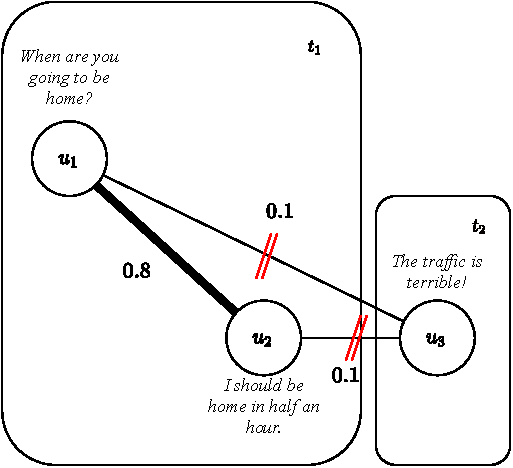
\includegraphics[width=0.7\textwidth]{graphSeg.pdf}
    \caption{Semantically different utterances have their connecting edge cut. The remaining clusters represent topics.\label{fig: graph seg}}
    \end{figure}

    \subsection{Bayesian Models}
    Some segmentation techniques rely on Bayesian models, assuming that the words in each $t_i$ are drawn from a distribution of words related to $t_i$. Maximising the observation likelihood yields the segmentation\cite{eisenstein2008bayesian}. The Bayesian framework then allows incorporating additional features such as particular phrases that can indicate a change in topic, such as "\textit{anyways}". Examples include \cite{purver2006unsupervised}\cite{eisenstein2008bayesian} and \cite{nguyen2012sits}, in which all authors have published their code.